\Lecture{Jayalal Sarma}{September, 08 2015}{21}{Structure of automorphism
groups for degree-$d$ graphs}{Sanjay Ganapathy}{$\gamma$}{K Dinesh}

In the previous lecture, we were interested in finding the generating set for
the automorphism group of $X$ which is given to be a graph bounded by maximum
degree 3. We in turn reduced this problem to solving the set stabilizer
problem for the special case where the group is a 2-group (that is $|G|$ =
$2^{k}$). 
%Given $G$, a $2$-group acting on $\Omega$ and $\Delta \subseteq
%\Omega$, find the generating set of setstab ($\Delta$). 
In order to solve the
set stabilizer problem for this group, first we shall characterize the
structure of automorphism groups for graphs with maximum degree $d$.

\begin{definition}[Composition Series]
For group G, a sequence of subgroups $G_{1}$, $G_{2},\ldots, G_{k}$ of $G$ is
said to be a composition series if,
\[ G = G_{0} \triangleright G_{1} \triangleright G_{2} \ldots
	\triangleright G_{k} = \{identity\} \]
and $\forall$ i, $G_{i+1}$ is a maximal strict normal subgroup of $G_{i}$. 
We call $G_{i+1} / G_{i}$ as composition factor.
\end{definition}

\begin{claim}
If a graph $X$ has maximum degree $\leq d$ and is connected, then $Aut_{e}(X)$
has a composition series with quotient groups isomorphic to $S_{d-1}$.
\end{claim}
Here $S_d$ denotes symmetric group on a set of size $d$.
However our interest is in the case when $d = 3$ and $Aut_{e}(X)$ is a
$2$-group. We will make use of Sylow's theorem to prove the existence of a
composition series for such a group where the size of each subgroup $G_{i}$
will be $2^{k - i}$ where $k$ is such that $|G| = 2^{k}$. 

\section{Sylow's Theorem}

\begin{theorem}[\textbf{Sylow's Theorem}] \label{thm:sylow}
If G is a group of size $p^{m}r$ where p is a prime and r is such that gcd (p,r) = 1, then $\exists$ H, such that $H \leqslant G$ and $|H|$ = $p^{m}$
\end{theorem}

However, this version of Sylow's theorem is not directly applicable to our problem, since in our problem, $|G| = 2^{k}$. Instead, we prove this restated version of Sylow's theorem.

\begin{theorem}
If $p^{l} \; | \; |G|$ then there exists a subgroup of size exactly $p^{l}$ for G.
\end{theorem}

\begin{proof}

Consider $|G|$ = $p^{m}r$ where $p^{k}$ divides r but $p^{k+1}$ does not divide r.

Consider the set $\Omega$ = \{ set of all subsets of G of size $p^{m}$ \}. Note this is not the $\Omega$ referred to at the starting of the lecture.

Action of g $\in$ G on any subset of size $p^{m}$ (assume action by left multiplication) will take the subset to some other subset of size $p^{m}$, that is it will be another element belonging to $\Omega$.

Consider A $\in$ $\Omega$, that is A is such that A $ $ G and $|A|$ = $p^{m}$.

$$ A^{g} = \{\; ga\; | \; a\; \in \; A \;\} $$
We know that
$$ |\Omega| = {p^{m}r \choose p^{m}} $$

\begin{theorem}[\textbf{Lucas's Theorem}]
If there is a prime p and positive integer r, such that gcd (p,r) = 1, then p $\nmid$ ${p^{m}r \choose p^{m}}$
\end{theorem}

This can be extended for the case where gcd (p,r) $\neq$ 1, as follows.
\begin{theorem}
If there is a prime p and positive integer r such that $p^{k} \;|$ r and $p^{k+1}$ $\nmid$ r, then $p^{k+1}$ $\nmid$ $p^{m}r \choose p^{m}$. 
\end{theorem}
\begin{proof}
The proof is quite simple. We just have to expand the term $p^{m}r \choose p^{m}$
\[  {p^{m}r \choose p^{m}} = \frac{p^{m}r \times (p^{m}r - 1) \times (p^{m}r - 2) \ldots \times (p^{m}r - (p^{m} - 1))}{p^{m} \times (p^{m} - 1) \times (p^{m} - 2) \ldots \times (p^{m} - (p - 1))} \]
We directly observe a natural numerator-denominator pair structure emerge. We know $p^{k}$ divides r. So, we just have to prove p does not divide the remaining number. Consider any numerator-denominator pair:
$$ \frac{p^{m}r - i}{p^{m} - i} $$
If $p^{\alpha}$ divides the numerator, we know $\alpha$ is definitely less than m because $i < p^{m}$, and $p^{m}$ cannot divide the numerator. So, if $p^{\alpha}$ divides the numerator, we observe that it will also divide the denominator. This follows from the observation that $p^{m}$ is divisible by $p^{\alpha}$ and so i must also be divisible by $p^{\alpha}$. Therefore $p^{m} - i$ is also divisible by $p^{\alpha}$. Thus p does not divide the remaining number and so $p^{k+1}$ does not divide $p^{m}r \choose p^{m}$. 
\end{proof}

Consider $\theta_{1}$, $\theta_{2}, \ldots , \theta_{K}$ to be the orbits of $\Omega$.
\[ \implies |\Omega| = |\theta_{1}| + |\theta_{2}| + \ldots + |\theta_{K}| \]
Since $p^{k+1}$ does not divide LHS, there exists at least one $i$ such that $p^{k+1}$ does not divide $|\theta_{i}|$. Since $A \in \theta_{i}$, orbit(A) = $\theta_{i}$.

Consider the pointwise stabilizer of A, $G_{A}$. We know from orbit-stabilizer lemma that
\[ |orbit(A)| \times |G_{A}| = |G| \]

$p^{m+k}$ divides the RHS. We know $p^{k+1}$ does not divide orbit(A). Therefore $|G_{A}|$ must be divisible by $p^{m}$. We'll now proceed to show that $|G_{A}|$ is in fact equal to $p^{m}$.

\begin{claim}
\[ |A| \geq |G_{A}| \]
\end{claim}

\begin{proof}
Suppose $|G_{A}|$ $>$ $|A|$. We know any element $g \in G_{A}$ stabilizes A, that is every element A is mapped to some other element in A, by action of $g$ by left multiplication. Let's take an element $g_{i}$ belonging to $A$. There are at most $|A|$ different elements that $g_{i}$ can go to. Since $|G_{A}| > |A|$, by pigeon hole principle we have that there exists at least 2 elements, say $g_{j}$ and $g_{k}$ belonging to $G_{A}$ such that they map $g_{i}$ to the same element say $g'$.
\[ g_{j}  g_{i} = g_{k}  g_{i} \]
By right multiplication with $g_{i}^{-1}$ on both sides, we will get that $g_{j}$ and $g_{k}$ are in fact equal. Thus, we arrive at a contradiction.
\end{proof}

Since $|A|$ = $p^{m}$, this implies \[ p^{m} \; | \; |G_{A}| \text{ and } p^m
\geq |G_{A}| \] Therefore $|G_{A}| = p^{m}$. Thus for any $p^{l}$ such that
$p^{l}$ divides $|G|$, we can prove the existence of a subgroup of size
$p^{l}$.

Coming back to our original problem of proving the existence of a composition
series for $Aut_{e}(X)$, since this is a $2$-group of size $2^{k}$, by Sylow's
theorem (Theorem~\ref{thm:sylow}) we know that a normal subgroup of size $2^{k-1}$
exists for $Aut_{e}(X)$. We can inductively extend this proof to each
subgroup, $G_{i}$ and thus prove the existence of a composition series.

In general, for any group $G$, $G \in B_{d}$ if there exists a chain of normal
subgroups such that each composition factor is isomorphic to $S_{d-1}$. We
call such a group to be structured. For the trivalent graph case, $d = 3$ and
hence the composition factor is isomorphic to $S_{2}$, which is what we have
shown.
\end{proof}

\section{Structure Forests}

We will solve the problem of finding a generating set for $\setstab (\Delta)$
using a recursive algorithm on a structure tree.

\subsection{Motivating Structure Trees}
Consider the same complete binary tree of depth $k$ we had used while
motivating groups and transitive actions, where we consider the existence of a
group $G$ such that $G \leqslant S_{n}$ and $G$ acts transitively on $\Omega$,
where $\Omega$ is the set of leaves. Each internal node of the tree can be
thought of as corresponding to a subset of $\Omega$, which is a block. In
general, when we have two vertices $u$ and $v$ such that $u$ is the child of
$v$, the following condition holds: \begin{center}
there does not exist a $\Delta$ such that $\Delta_{u}$ $\subset$ $\Delta$ $\subset$ $\Delta_{v}$ 
\end{center}
We call $u$ as a child of $v$ if $\Delta_{u}$ is a maximal block in $\Delta_{v}$.
\begin{observation} 
When $G$ is general, you get a structure forest, with each tree corresponding to an orbit. This follows from the fact that G acts transitively on an orbit by definition. 
\end{observation}

In the next lecture, we'll formally define structure forests and use them to formulate a recursive solution for the restricted set stabilizer problem and prove that the running time of the algorithm is bounded by a polynomial for $d$ degree graphs.

\Lecture{Jayalal Sarma}{September, 09 2015}{22}{Solving Restricted Set
Stabilizer Problem}{Sanjay Ganapathy}{$\gamma$}{K Dinesh}

We will formalize the notion of structure forests that we motivated in the last lecture.

\section{Structure Forests}
\begin{definition}[Structure Forests]
Given a group $G$ that acts on $\Omega$, consider a forest 
with a trees $T$  such that 
\begin{enumerate}
\item each tree in the forest corresponds to one orbit.
\item leaves as the elements of $\Omega$, internal nodes correspond to blocks and root correspond to orbit.
\item vertex $u$ in $T$ is a child of vertex $v$ if $\Delta_{u}$ is a maximal block in $\Delta_{v}$.
\end{enumerate}
\end{definition}

\begin{figure}[htp!]
	\centering
	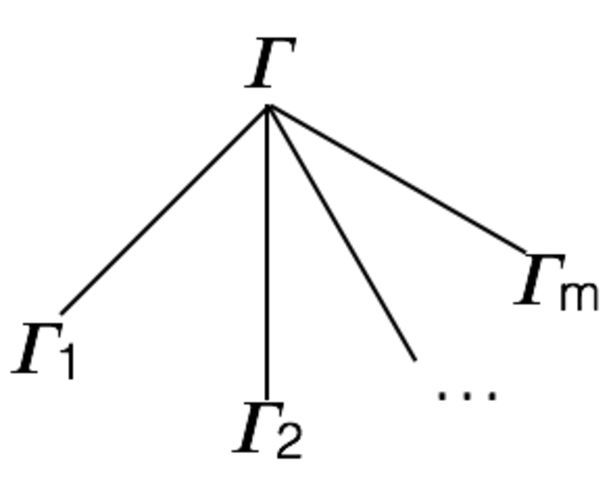
\includegraphics[scale=0.5]{images/structuretree.pdf}
	\caption{Each $\Gamma_{i}$ is a maximal block in $\Gamma$.}
	\label{fig:maxblocks}
\end{figure}

\begin{claim}
Action of G on the set ${\Gamma_{1}, \Gamma_{2}, ..., \Gamma_{m}}$ is primitive.
\end{claim}
\begin{proof}
Consider action of $G$ on the set $\{1, 2, 3, ... m\}$. Suppose there was a non-trivial block $\delta \subset \text{ \{1, 2, ... m\}}$ and$|\delta| 
\neq 1 $. Let $B$ be defined as $ B = \bigcup_{i \in \delta} \Gamma_{i} $
Note that, $B$ is a block in $G$ acting on $\Omega$. 
Hence for any $i \in \delta$, $B$ forms a non-trivial block as $\Gamma_{i}$ $\subset$ B $\subset$
 $\Gamma$. But then $\Gamma_i$ is no longer maximal block of $\Gamma$  contradicts the existence of the edge $\Gamma$ to  $\Gamma_{i}$.
\end{proof}

Consider the partition of $\Omega$ into its orbits. This partition can be computed efficiently by algorithm~\ref{alg:orbit_alg}. 
$$ \Omega = \Omega_{1} \cup \Omega_{2} ... \cup \Omega_{k} $$
We make the following observation which gives a divide and conquer strategy.
\begin{observation}
It suffices to find the setstab of $\Delta\cap\Omega_{i}$ separately and take the union.
\end{observation}

This is because, there does not exist a group element $g$ which can take any element belonging to $\Omega_{i}$ to $\Omega_{j}$ where $i \neq j$, by virtue of the two elements being in different orbits. Thus when $\Delta$ is stabilized, elements belonging to an orbit are also constrained to remain in the same orbit.

Thus we have reduced our original problem to finding the generating set of $\Delta\cap\Omega_{i}$. Here on, we will focus on one orbit and refer to it as $\Omega$ and $\Delta\cap\Omega$ as $\Delta$. Note that action of $G$ on $\Delta \cap \Omega_1$ is transitive as theses are points inside an orbit.

\section{Algorithm for computing setstab($\Delta$)}
Consider the structure tree for this action.
\begin{figure}[htp!]
	\centering
	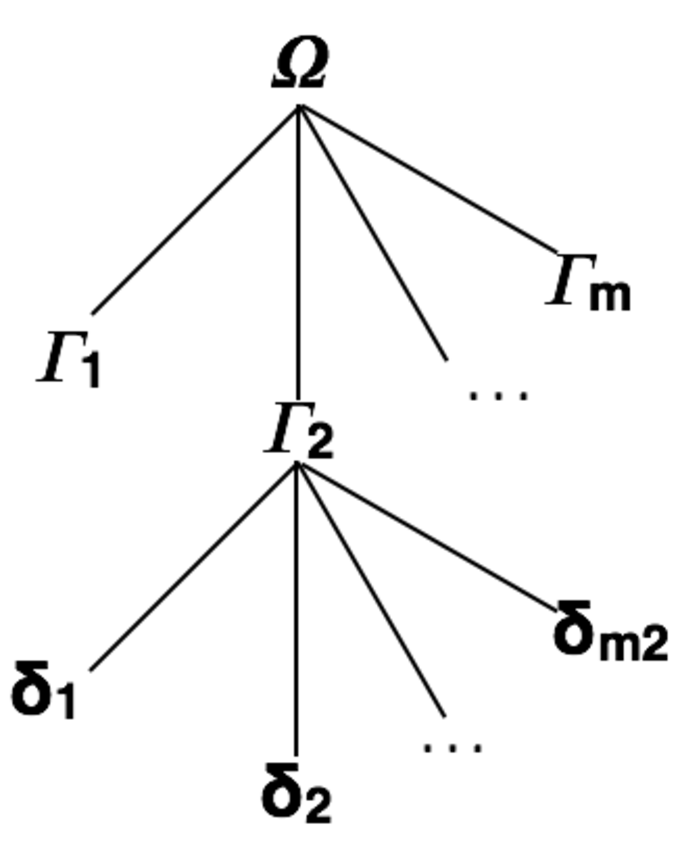
\includegraphics[scale=0.3]{images/setstabalg.pdf}
	\caption{Structure tree for one orbit of $\Omega$ under the action of $G$.}
	\label{fig:structurestree}
\end{figure}
Let $H$ = \{ $g$ $\in$ $G$ $|$ $\forall$ $i$ $\Gamma_{i}^{g}$ = $\Gamma_{i}$ \}. $H$ is the setwise stabilizer of $\Gamma_{i}$. This means we can write $G$ in terms of the cosets of $H$. Let there be $k$ cosets and $\tau_i$ denote the coset representatives. Hence,
\begin{figure}[htp!]
	\centering
	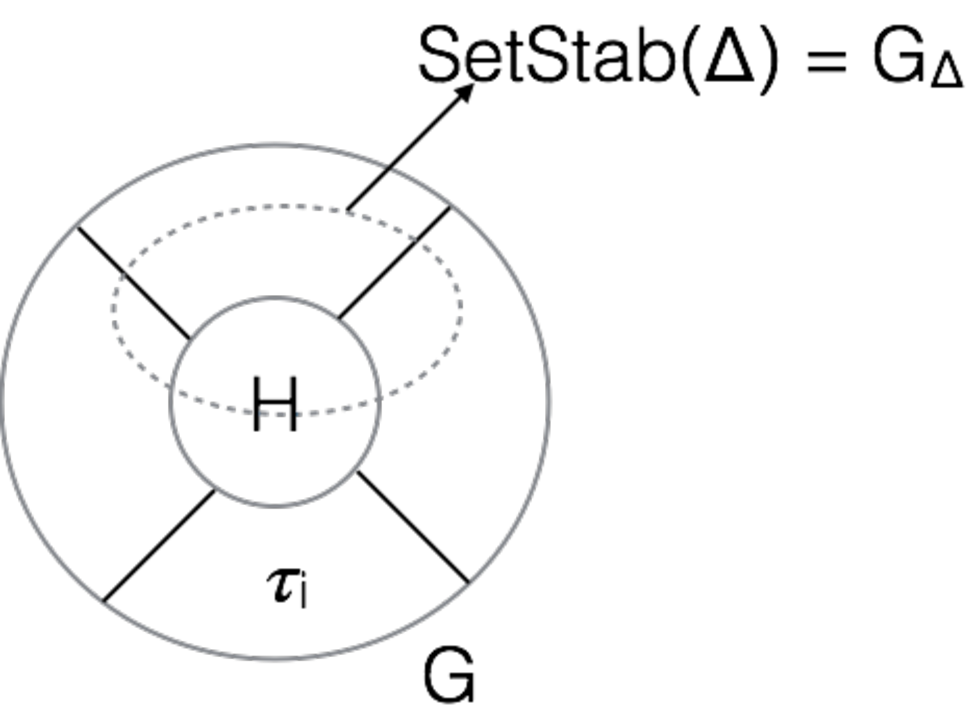
\includegraphics[scale=0.45]{images/setstabgroup.pdf}
	\caption{Set Stabilizer group of $\Delta$ in G and the cosets of $H$, which is the setwise stabilizer of $\Gamma_{i}$.}
	\label{fig:setstabgroup}
\end{figure}

\[ G =  \bigcup_{i=1}^kH\tau_{i} \]
\[ G_{\Delta} = \bigcup_{i=1}^k(H\tau_{i})_{\Delta} \]

We need to find the elements in each coset of $H$, which stabilizes $\Delta$. This leads to a natural recursive formulation which we formalize below. 

\begin{problem}[Generalized Set Stabilizer]
Given $\Delta$, $H$ and $\sigma$, such that $H$ stabilizes $\Omega'$, where $\Omega'$ $\subseteq$ $\Omega$, find $(H\sigma)_{\Delta}$. 
\end{problem}
If we visualize $\Delta$ to be a $2$ colouring on the elements of $\Omega$, then we can write
\begin{center}
SetStab (H, $\sigma$, $\Omega'$) = \{$h$ $\in$ $H\sigma$ $|$ $\forall$ $\omega$ $\in$ $\Omega' \text{ $\omega$ and $\omega^{h}$ has the same colour}$\}
where $\Omega'$ is one of $\Gamma_{i}$.
\end{center}

Therefore, we need to recursively solve SetStab($\Gamma_{i} \cap \Delta, \sigma$), for each level of the tree. To show that this algorithm runs in polynomial time, we make use of the following bound.

\begin{theorem}[Babai, Cameron, Palfy]
If $G \leqslant S_{n}$ is a structured group, then $|G|$ is bounded by $n^{c}$  for some constant c.
\end{theorem}

We have already proved that $Aut_{e}(X)$ is a structured group, for a d-degree bounded graph. Thus, we can use this theorem to show that $|G| \leq n^{cd}$. Thus the number of nodes in the tree is polynomial and number of coset representatives is also polynomial since the size of the group itself is bounded by a polynomial. Thus, since the recursion only visits each node of the tree once, and the computation per node is bounded by a polynomial, the entire algorithm is of polynomial order.More precisely, we can show that we can solve the graph automorphism problem in $O(n^{d^{2}})$ time.

In the next lecture, we will try to refine the trivial brute force algorithm of finding a graph isomorphism between $2$ graphs $X_{1}$ and $X_{2}$ and develop an algorithm which runs in $O(n^{n^{\frac{2}{3}}})$.

